\chapter{Electromechanical Design} % (fold)
\label{cha:design}
The electromechanical design of the lower body biped involves several key considerations which impact the performance of the finished product. The complete process consists of selecting the appropriate drivetrain components (electric machines) and designing the mechanical chassis. The primary design objective is to produce enough mechanical power for the robot to achieve walking. The secondary design objective is to keep the overall weight low and shift the center of mass (COM) position as high as possible. 

The selection of electromechanical components which compose the drivetrain system will be used to address the primary objective. These drivetrain components include electric machines (DC motors) and adequate gearing which will provide the reduction ratio required to meet the design specifications. Once the primary objective is addressed and the drivetrain components have been selected, the secondary objectives will be satisfied by adjusting the mechanical structure and manipulating placement of components. This approach provides the means to meet design constraints such as reducing the overall mass of the system or shifting the COM position higher in the structure.

%======================================================================
%   D Y N A M I C  M O D E L I N G
%======================================================================

\section{Dynamic Modeling} % (fold)
\label{sec:chassis}

A dynamic model of the proposed system must be developed and analyzed under normal operating conditions to determine the effect of forces acting on the system and torques experienced at each of the joints. The forward or direct dynamic model is a mathematical system which provides a transformation from the joint torques to the resulting joint positions, velocities and accelerations. That is, it provides the relationship:

\begin{equation}
	\ddot{\vec{q}} = f(\vec{\tau})
\end{equation}

Given this model, a dynamic simulation environment can be designed to determine the torques experienced at different joints on the biped robot while undergoing a gait cycle. This estimate can form the basis of the initial drivetrain specifications from which motors and gearing can be selected for the electromechanical design. An important consideration in this model is the implementation of a contact force that is experienced during the stance phase of the gait cycle. The ground reaction forces exerted on the robots feet have a significant impact on the dynamics of each joint. Since the stance phase makes up approximately 60\% of the gait cycle, the effects of these ground reaction forces have to be incorporated for an accurate simulation. 
% section overview (end)

\subsection{Forward Dynamics} % (fold)
\label{sec:forward_dynamics}

The overall dynamics of any multibody robotic system can be expressed by the following equation of motion: 

\begin{equation}
	\label{eq:motion}
	A(q)\ddot{\vec{q}} + C(\vec{q},\dot{\vec{q}})\dot{\vec{q}} + g(\vec{q}) = \Gamma
\end{equation}

Where $A(q)$ is the $n$ x $n$ inertia matrix, $C(q,\dot{q})$ is the centripetal and Coriolis terms and $g(q)$ is the gravity term. On the right hand side, $\Gamma$ is $n$ x 1 force vector which describes the torque at each of the joints in the system. The $\ddot{q}$ is also a $n$ x 1 vector representing the generalized coordinates of the multibody system. For most cases, the number of generalized coordinates $n$ is equivalent to the number of degrees of freedom. However, for the case of humanoid robots with floating bases there is an additional 6 degrees of freedom which represent the movements of the base \cite{Perrin:1997wn}. Therefore, for the 14 DOF lower body system there is a total of $n = 20$ generalized coordinates. In order to incorporate the effects of contact forces at both feet of the biped robot, the equation of motion presented in Equation \ref{eq:motion} is modified as follows: 


\begin{equation}
	\label{eq:motion2}
	\begin{bmatrix} A_{11} & A_{12} \\ A_{21} & A_{22} \end{bmatrix} 
	\begin{bmatrix} \ddot{\vec{q}}_{joints} \\ \ddot{\vec{q}}_{base} \end{bmatrix} + 
	\begin{bmatrix} b_{1} \\ b_{2} \end{bmatrix} = 
	\begin{bmatrix} \vec{\tau} \\ 0 \end{bmatrix} + 
    J^{T}\vec{F}_{left} + J^{T}\vec{F}_{right}
\end{equation}

Where the generalized acceleration vector $\ddot{q}_{joints}$ represents the $n$ DOF joint motion and $\ddot{q}_{base}$ is for the 6 DOF base motion. The gravitational and Coriolis terms are combined into the $\vec{b}$ vector. Finally, $J$ is a 6 x $n$ Jacobian matrix which relates the joint space variables to the work space variables. The force vectors $\vec{F}_{left}$ and $\vec{F}_{right}$ represent the contact force felt at the left and right foot, respectively. With this modification of the equation of motion, the external forces felt during the stance phase can be incorporated into the dynamic model of the overall system. The method of calculating the magnitude of the force itself depends on the contact model used for the system. Therefore, Equation \ref{eq:motion2} represents the complete dynamics of the biped robot with $n = 20$ generalized coordinates.

One method of computing a direct dynamic model for the biped robot is through the use of the Recursive Newton-Euler (RNE) algorithm. This algorithm computes the inverse dynamics model iteratively in order to arrive at a final solution for the direct dynamics \cite{Perrin:1997wn}. The RNE algorithm serially traverses through the kinematic chain to perform calculations using Newtonian mechanics. The first pass of the algorithm starts at the base link and traverses down the serial chains of the left and right legs calculating the kinematics. The second pass starts at the end of the serial chain(s) and works back up to the base link calculating the effect of dynamics. As a result, the RNE algorithm is capable of calculating the torques located at each joint and the 6 dimensional forces and moments felt by the base joint. Using this algorithm, the direct dynamics model can be computed by reformulating Equation \ref{eq:motion}. The pseudocode listed in Appendix \ref{sec:rne_direct_dynamics} describes the procedure for computing the direct dynamics model by utilizing the RNE formulation.

% section forward_dynamics (end)

\subsection{Contact Modeling} % (fold)
\label{sec:contact_modelling}

\begin{figure}[!ht]
	\begin{center}
    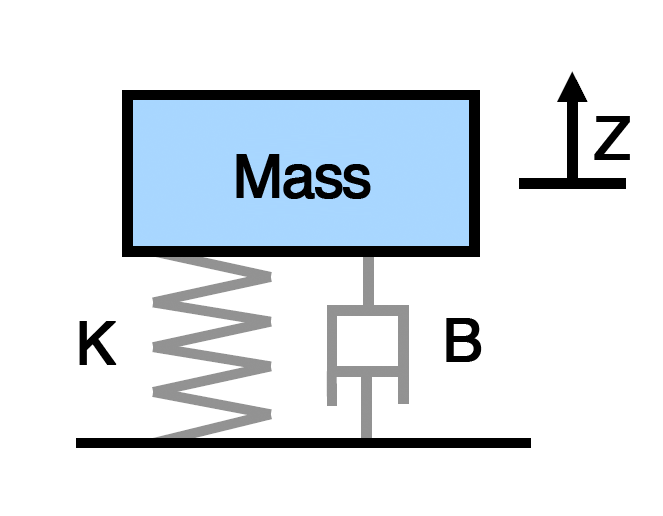
\includegraphics[width=100mm]{fig/ch5/springdamper.png}
	\end{center}
  \caption{System diagram of spring-damper contact model used in dynamic simulations.}
\end{figure}

One challenging aspect of dynamic simulations is to accurately model the effects of external forces on the system during the stance phase. To emulate the ground reaction forces during this period of the gait cycle, a contact model is used to generate an approximation of the contact force. For the purposes of this project, a simple spring-and-damper contact model is used. For the sake of simplicity, both feet of the biped are modelled as point contacts which experience a normal force proportional to the output given by Equation \ref{eq:contactf} when in contact with the ground. 

\begin{equation}
	\label{eq:contactf}
	\vec{F}_{contact} = B\vec{\dot{x}} + K\vec{x}
\end{equation}


To incorporate the effects of the contact model into the existing dynamic model, the contact force as described in Equation \ref{eq:contactf} is injected into the RNE algorithm between the end of the first pass and the start of the second pass. In other words, at the beginning of the second pass the external force used as an initial condition is modified to equal the amount of force produced by the spring damper model. Due to the serial nature of RNE, this force traverses up the kinematic chains for each leg and is finally resolved at the base. Alternatively, the equivalent force can be substituted into the overall system dynamics represented in Equation \ref{eq:motion2} for $F_{left}$ and $F_{right}$. Both approaches will yield identical results as the force is resolved into different parts of the biped robot. 

% section contact_modelling (end)

\subsection{Kajita's Matlab Toolbox} % (fold)
\label{sec:kajita_s_matlab_toolbox}
A quick and easy tool for setting up the dynamic simulations was to use an existing robotics toolbox in Matlab. Professor Shuuji Kajita packages a simple Matlab toolbox along with his textbook on humanoid robotics which provided a platform to get started with setting up the dynamic models \cite{kajitatxt}. 

\begin{figure}[!ht]
	\begin{center}
    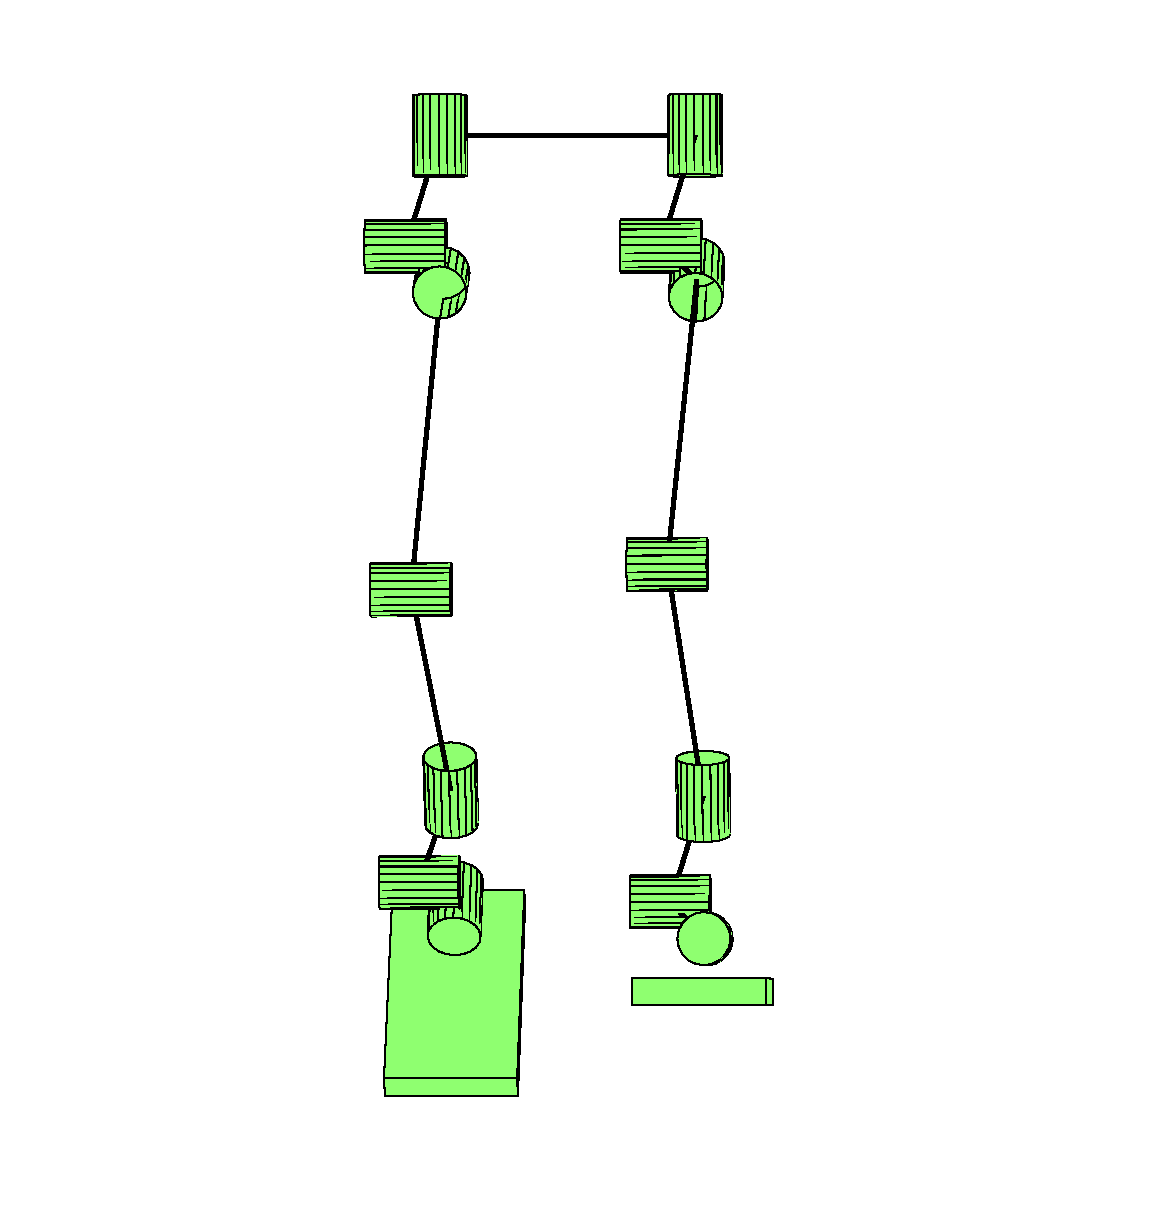
\includegraphics[scale=0.6]{fig/ch5/ulinkdrawn.eps}
	\end{center}
  \caption{Screenshot of robot structure drawn from uLINK definition.}
\end{figure}

The Matlab toolbox provides a series of scripts and functions which perform standard operations on a robotic structure (i.e. forward or inverse kinematics). Each of the functions in the toolbox revolve around the use of an object definition of the robot structure known as \texttt{uLINK}. The kinematic description for each of the links in the robot are defined as part of this \texttt{uLINK} structure using a convention specified in the accompanying textbook. An external application was written in Microsoft's .NET environment which interfaced with the API for the 3D CAD package (SolidWorks) in order to automatically generate the corresponding \texttt{uLINK} representation in Matlab code. 

Once the \texttt{uLINK} structure is established, any of the preprogrammed routines in the toolbox can be used to manipulate the kinematic structure. The most important functionality bundled with the toolbox is the direct dynamics routine. This is simply an implementation of the RNE algorithm described in Section \ref{sub:recursive_newton_euler}. However, in its original implementation the direct dynamics omits athe effects of any external forces which is necessary for the stance phase of the gait cycle. Therefore several modifications were required in order to emulate the effect of ground reaction forces through a contact model to properly size electromechanical components to withstand the impacts. 

While the toolbox provides a stable starting platform for setting up the dynamic simulation, several modifications were required in order to incorporate the effects of a contact model. The key modification required was to implement the effect of contact forces experienced by the stance leg throughout the gait cycle. Since the direct dynamics calculations were performed was based on the RNE algorithm, the modification was fairly straight forward. The initialization phase of the backwards pass in the routine (from the end of the serial kinematic chains back up to the base link) was modified according to the following code: 

\lstinputlisting{code/kajitamod.m}

Where the variables \texttt{Kr} and \texttt{Br} represent the spring and damper coefficients in the spring-damper contact model. \texttt{RCONTACT} is simply a constant link number representing the point contact foot. The velocity due to the point foot coming in contact with the ground (\texttt{vr}) is recomputed by considering the original velocity (\texttt{vo}) and the cross product between the position of the foot (\texttt{uLINK.p}) and angular velocity (\texttt{uLINK.w}). The resulting normal force is computed and injected into the backwards pass if the foot position is below the ground level (condition shown in line 1). 

Using this conditioning, the initialization sequence of the backwards chain simply checks for the position of each foot in world coordinates to determine whether ground contact is present. The ground throughout the simulation is assumed to be represented by the $z = 0$ plane. Therefore, for any value of $z > 0$ the foot is not in contact with the ground and subsequently $z \leq 0$ represents contact is present. In the situation where contact is present, a ground normal force proportional to the output of the spring-damper system is injected into the system. Due to the recursive nature of the RNE algorithm, this force back-propagates through each of the links in the serial chain until it is ultimately resolved at the terminating base link.
% subsection modifications (end)

% section kajita_s_matlab_toolbox (end)

\subsection{Gait Estimation} % (fold)
\label{sec:gait_estimation}
	
In order to emulate the operating conditions for the lower body biped robot once it is built, the dynamic simulation must incorporate the effects of executing a gait cycle. This allows for investigation into the external  forces experienced by the robot structure while walking. 
	
One method of emulating the normal operating conditions is to estimate the effects by using human gait. While it is highly ambitious that a walking robot will be able to achieve the performance of human-like walking, it provides a basis to from which the initial selection of electromechanical components can emerge. The goal is to extract the kinematic parameters experienced by the human limbs while walking and impose similar conditions in the dynamic simulation. Given these constraints, the inverse dynamics problem can be solved in order to obtain the joint torque estimates during various points in the gait cycle. Coupled with the modifications to emulate contact forces during the stance phase, this simple dynamic simulation provides a quick and easy way to estimate the torque loading at the joints to develop initial design specifications. 
	
In order to use kinematic parameters from human gait, data published from the 2008 Dynamic Walking conference was used \cite{dw2008}. The published data used several sensors to measure the joint angles and velocities of lower body human limbs under several gait cycle speeds (i.e. fast walk, slow walk, normal walk, etc). During the data collection, sensors were strategically placed such that key information such as the knee yaw and hip pitch was captured. This raw sensory data was imported into the Matlab environment using a 3D motion analysis toolbox known as BodyMech \cite{bodymech}. This information was incorporated into the dynamic simulation by enforcing the joint angles, velocities and accelerations from each captured frame of the reference dataset. By accomplishing this, the \texttt{uLINK} robot structure which modelled the dynamic parameters (mass, link inertias) with the captured 3D kinematics of human gait. 

An experiment was devised in the Matlab environment which used a combination of the BodyMech toolbox and Kajita's toolbox. The BodyMech toolbox was used to extract the frame-by-frame 3D kinematic parameters as a human executed the gait cycle. These parameters were processed and stored in order to be played back on the robot model defined by the \texttt{uLINK} structure. The Matlab script provided in Appendix \ref{sec:gait_analysis_script} was used to load the 3D kinematic parameters from each frame and apply the transformed equivalent on the robot structure. To compensate for the differences in size between humans and the small biped, the joint velocities and accelerations were scaled by selecting a different reference gait speed from the published data set. 
	
Once the parameters were applied, the inverse dynamics routine was executed in order to determine the torques at each joint in the structure as result of the gait dynamics. Note that the inverse dynamics routine was also modified to emulate the contact force effects experienced during the stance phase of the gait cycle. This process was repeated for each frame in the captured data and the results of robots kinematics and dynamics ($q$, $\dot{q}$, $\ddot{q}$ and $\tau$) were tabulated in CSV files for post processing. 
	
\begin{figure}[!ht]
	\begin{center}
	\begin{tabular}{cc}
	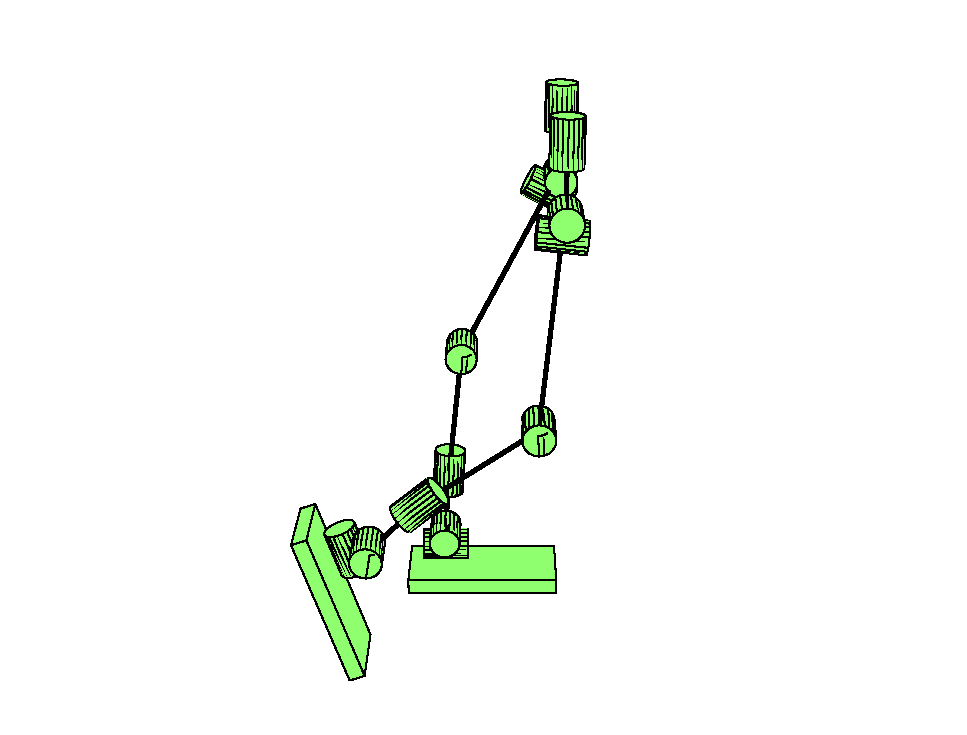
\includegraphics[scale=0.5]{fig/ch5/ulinkwalk1.eps} &
    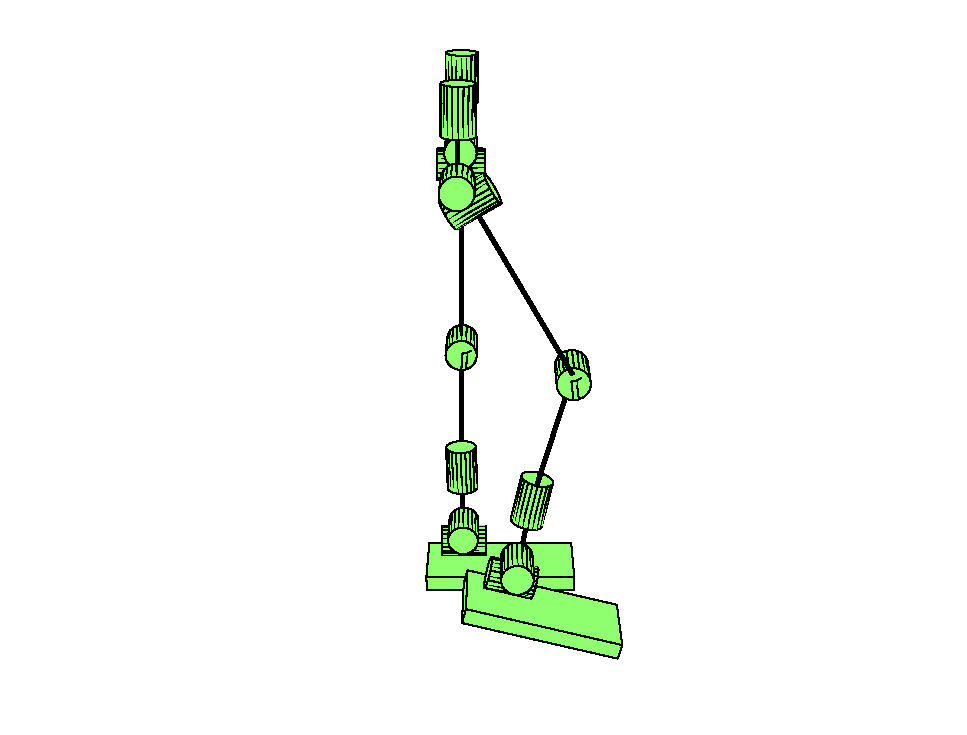
\includegraphics[scale=0.5]{fig/ch5/ulinkwalk.eps}
	\end{tabular}
	\end{center}
  \caption{Screenshot of gait analysis of uLink structure executing human-walk.}
\end{figure}
	
% section gait_estimation (end)


\subsection{Initial Design Requirements} % (fold)
\label{sec:initial_design_requirements}

\begin{figure}[!ht]
	\label{fig:gaitplot}
	\begin{center}
    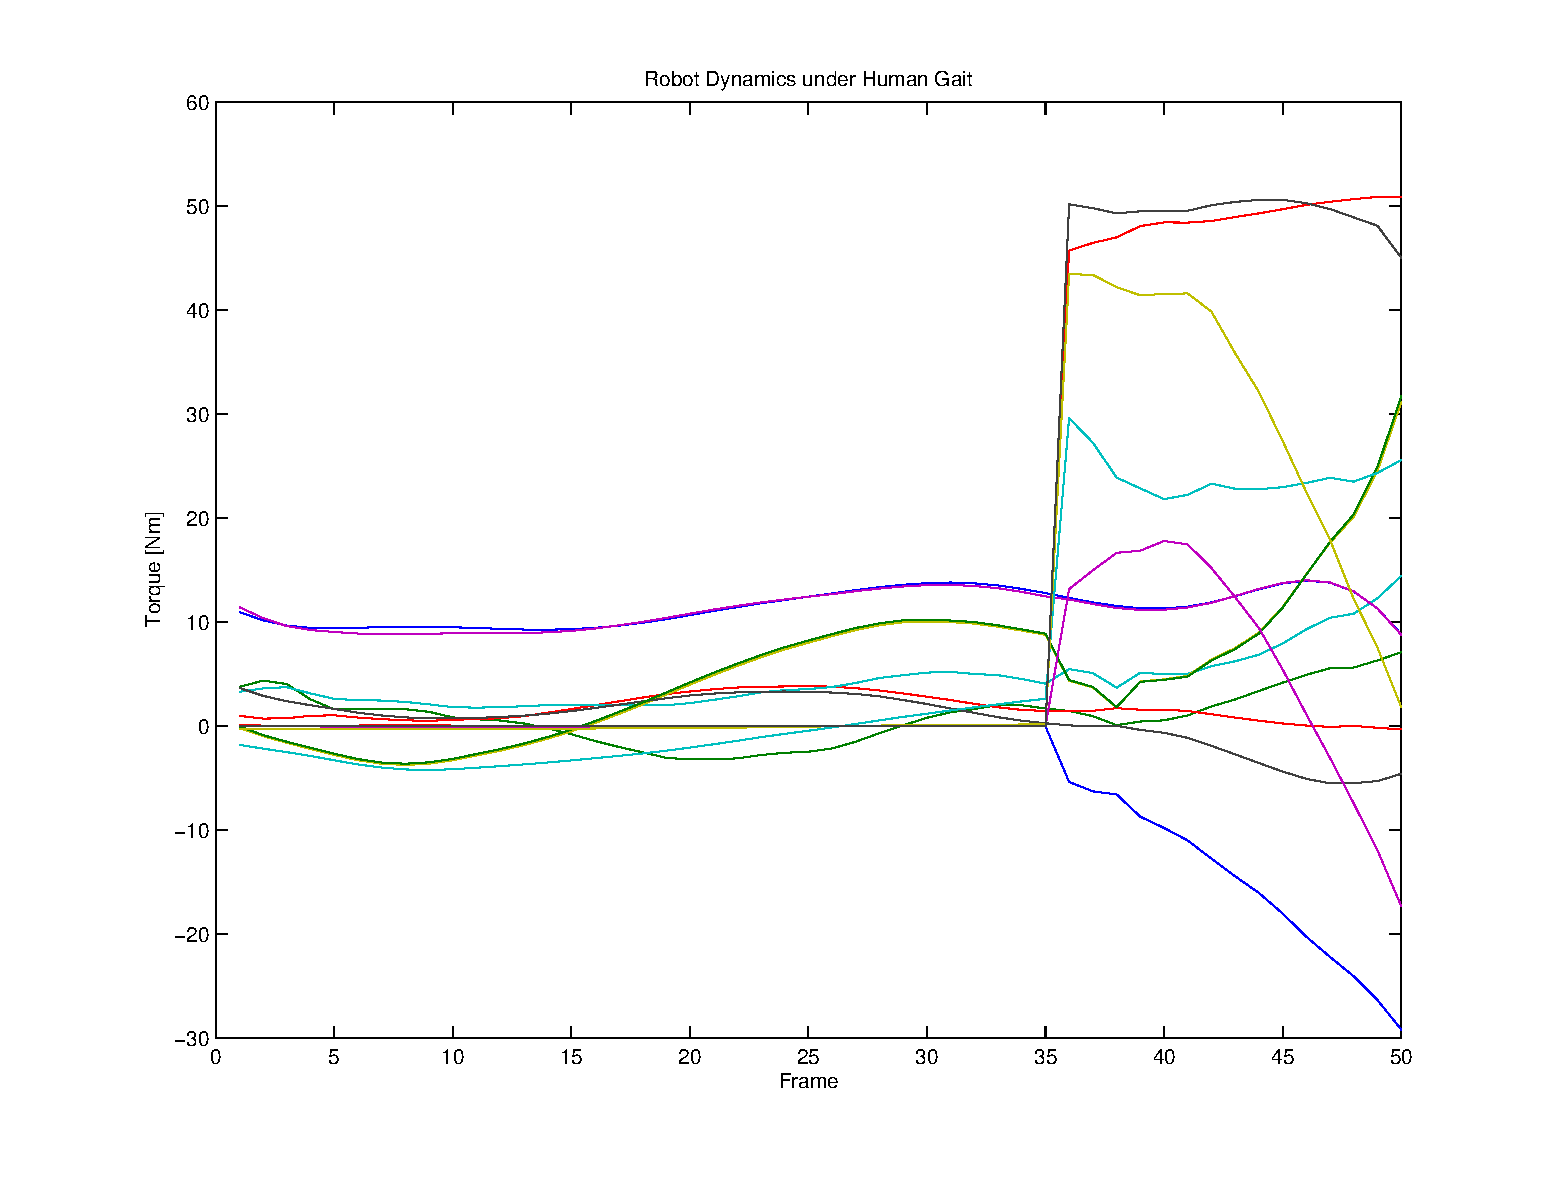
\includegraphics[scale=0.6]{fig/ch5/gaitplot.eps}
	\end{center}
  \caption{Joint torque profile during the execution of human-gait kinematics from reference data set.}
\end{figure}

The results of the dynamic simulations under human-gait analysis form the basis for the initial electromechanical components selection process. As expected, it was observed that the largest demands in torque loading on each of the joints occurred during the stance phase immediately after the heel strike event (refer to Frame 36 in Figure \ref{fig:gaitplot}). The torque demands at that instant spike immediately to almost 3x the steady state torque loading on the joints. While it is expected that a walking robot will experience large spikes in the torque demands such as the ones observed in the dynamic simulation, it is unreasonable to use only the peak torque values as the required specifications for design. 

\begin{table}[!ht]
  \centering
  \caption{Individual joint torque demands for each DOF in one leg.}
    \begin{tabular}{lcc}
    \addlinespace
    \toprule
    \textbf{Joint} & \textbf{Normal} & \textbf{Peak}\\
    \midrule
    Ankle Roll	&	13.824 Nm	&	14.021 Nm\\
    Ankle Pitch	&	4.395 Nm	&	7.923 Nm\\
	Ankle Yaw	&	3.858 Nm	&	3.858 Nm\\
	Knee Pitch  &	5.229 Nm	&	16.539 Nm\\
	Hip Roll	&	13.606 Nm	&	14.054 Nm\\
	Hip Pitch	&	10.081 Nm	&	38.295 Nm\\
	Hip Yaw		&	3.698 Nm	&	3.698 Nm\\
    \bottomrule
    \end{tabular}%
  \label{jointtable}%
\end{table}%


Since one of the secondary objectives is to keep the overall mass of the biped as low as possible, it is desirable to select smaller motors where the peak torque loading on the joints are outside of the allowable range of continuous operation. This is a reasonable estimate since the peaks are impulsive forces which only last for a short period of time. The practical approach for deriving specifications from the dynamic simulations is to analyze the continuous torque loading while the system undergoes the gait cycle while keeping the peak loading requirements as a secondary objective. 

While the torque demands vary from one joint to the next (see Table \ref{jointtable}), the results from the analysis are concatenated to obtain only a single set of design specifications. This also helps to limit the different types of motors selected from the manufacturer and greatly simplifies the electromechanical design process. The task of fine tuning the motor selection for each joint is left for future revisions. Therefore, the set of design specifications for the joint torques are summarized in Table \ref{tab:spectable}

\begin{table}[!ht]
  \centering
  \caption{Initial design specifications for electromechanical components.}
    \begin{tabular}{lcc}
    \addlinespace
    \toprule
    \textbf{Condition} & \textbf{Torque} & \textbf{Velocity}\\
    \midrule
    Normal & 14 Nm & 2.48 rad/s\\
    Peak  & 50 Nm & 6.82 rad/s \\
    \bottomrule
    \end{tabular}%
  \label{tab:spectable}%
\end{table}%

For the initial design consideration, the normal torque specification shown in Table \ref{tab:spectable} is obtained by taking an average of joint torque values during the swing phase. Since the ground reaction forces experienced during the stance phase produce large torques in a short period of time, the peak torque specification in Table \ref{tab:spectable} is obtained by selecting the highest torque value from all frames.

The contact model parameters (spring and damping coefficients) were observed to have a noticeable effect on the peak design specifications. Since the contact model only provides a crude approximation of the ground reaction forces that the real robot will experience, the final selected value was chosen to provide a peak torque which averages between the largest and smallest values. The final spring and damping coefficients used in deriving the design specifications were $K = 10000$ and $B = 100$, respectively.
% section chassis (end)


%======================================================================
%   D R I V E T R A I N  S E L E C T I O N
%======================================================================


\section{Drivetrain Selection} % (fold)
\label{sec:drivetrain}
The drivetrain selection process includes selecting the appropriate components which will transmit the torque required by the initial design specifications to the joints. The actual drivetrain components which are selected for this project are supplied by the Micromo Solutions part of the Faulhaber Group. The product catalog provided online was used as a reference tool for the drivetrain selection process. The electric machines used to generate mechanical power for the purposes of this project are coreless DC motors. As mentioned previously, the majority of the mass distribution in the robot system is attributed to the weight of the motors. Therefore, one of the design objectives for this project was to select a combination of motor and appropriately sized gearhead (also supplied by Micromo Solutions) to meet the design specification torque requirements while keeping the overall mass low. Therefore, the drivetrain selection process refers to the selection of appropriate coreless DC motor and matching gearhead which will meet the design requirements. 


\subsection{Mechanical Power Requirements} % (fold)
\label{sub:mechanical_power_requirements}
Similar to most large manufacturers of electric machines, Micromo Solutions provide a large catalog of DC motors which are aimed towards a large variety of applications. In order to narrow down the selection process into a subset of the motors which are applicable for the level of torque specified by the initial specifications, preliminary mechanical power calculations are performed. Recall that the mechanical power required by the drivetrain is specified by the required torque ($\tau$) and speed ($\omega$) of the motor: 

\begin{equation}
	P = \tau \times \omega
\end{equation}

The initial specifications for the drivetrain components listed in Table \ref{tab:spectable} list two values for the torque. As mentioned previously, designing the system to meet the peak torque requirements would yield significantly larger motors and increase the overall mass. Instead, it is desirable to design the system to meet the average (continuous) torque requirements and ensure that the system is capable of withstanding the large impulsive forces experienced at the impact points of the gait cycle. Therefore, the initial mechanical power requirement calculation is based on the normal or average torque loading on the joints (14Nm). While no speed requirements were specified in the initial design specifications, the tabulated kinematic and dynamic data collected from the dynamic simulation was used to compute the average speed experienced by the joints and the largest value was selected for the purposes of calculation. This provides a large buffer in the mechanical power considerations since not all joints are likely to experience such high speeds. The average speed calculated from the dynamic simulation was found to be 65RPM. Substituting these values along with the conversion factor for units: 

\begin{equation}
	P = \tau \times \omega = 14Nm \times 65RPM \times 0.1047 = 95.28W
\end{equation}

Using this value of mechanical power as a starting guide, the motor catalog is consulted to eliminate the majority of the solutions provided. Note that due to the assumptions placed in calculating this value, 95.28W represents an upper bound on the amount of power the design should be capable of providing. Therefore the potential solution candidates should be rated for the nominal power around the region of this value. 

% subsection mechanical_power_requirements (end)

\subsection{Torque-Speed Analysis} % (fold)
\label{sub:torque_speed_analysis}
The primary chart for analyzing and comparing different alternative solutions is through the use of a torque-speed plot. Given the structure of the motor specifications provided by Micromo Solutions, a spreadsheet was constructed in Microsoft Excel 2010 to automatically generate the torque-speed characteristic chart from the motor constants. These constants were pre-populated and the charts were generated on the fly. 

\begin{equation}
	\omega = \omega_{no-load} - k\tau
\end{equation}

The equations used to generate the torque speed relationships were fairly simple equations using the motor constants provided by the manufacturer on the specification sheets. The relationship between the torque of the motor and the speed of the revolving shaft is approximately linear so it is typically specified by a slope constant for the curve. While the constant $k$ is usually provided as a positive value, the slope of the torque-speed curve is negative (i.e. as the torque increases the speed decreases). 

\begin{figure}[!ht]
	\begin{center}
    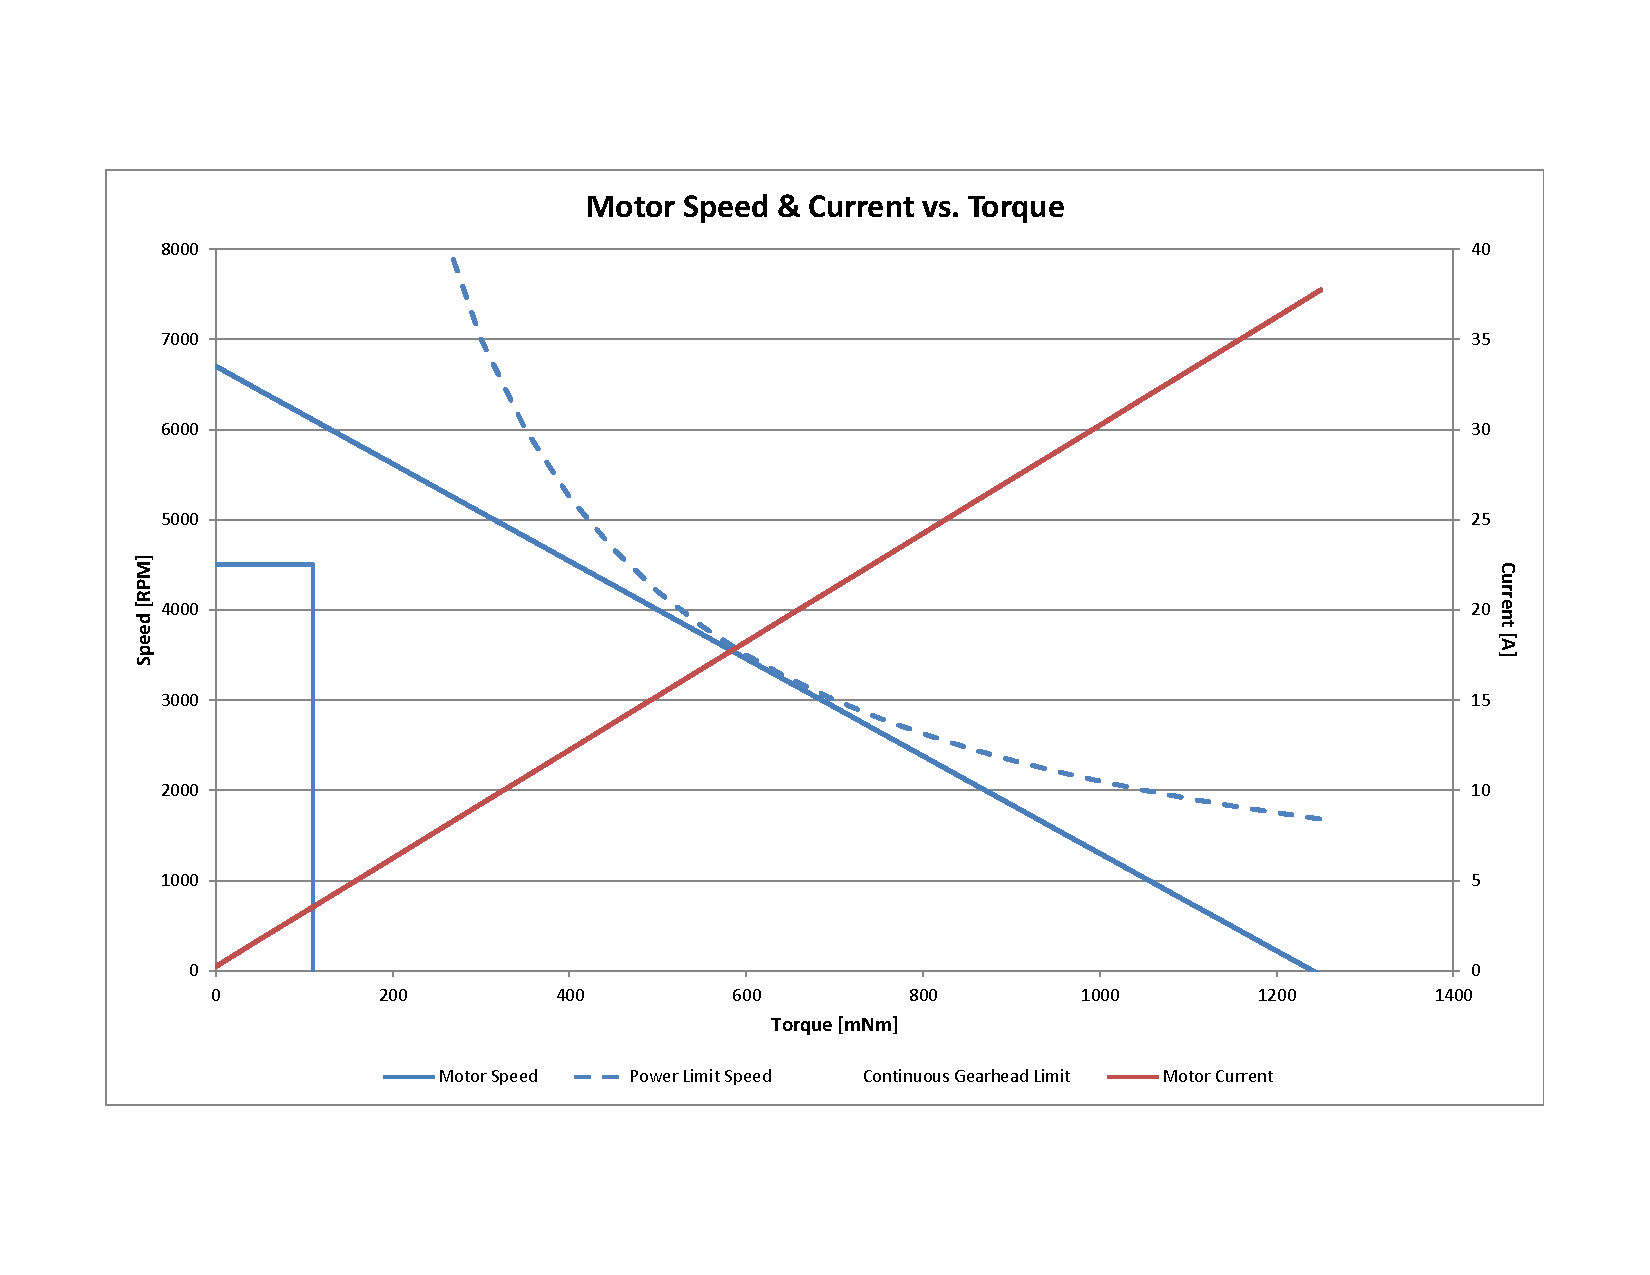
\includegraphics[scale=0.6]{fig/ch5/motor1.pdf}
	\end{center}
  \caption{Micromo 3257CR Coreless DC Motor: Speed and Current vs Torque}
\end{figure}

% subsection torque_speed_analysis (end)

\subsection{Power and Efficiency Analysis} % (fold)
\label{sub:power_and_efficiency_analysis}
Another key factor in comparing drivetrain components is the relationship between the power produced and the overall efficiency of the motor as a function of its torque. The efficiency curve compares the ratio of electrical power input to mechanical power output. While it is typically desirable to operate the motor at its peak efficiency, throughout the gait cycle the loading on the motors undergo a variety of changes so it is difficult to base the motor selection process based on this premise. However, it is desirable to ensure that the motor is reasonably efficient in the general region of operation. 


\begin{figure}[!ht]
	\begin{center}
    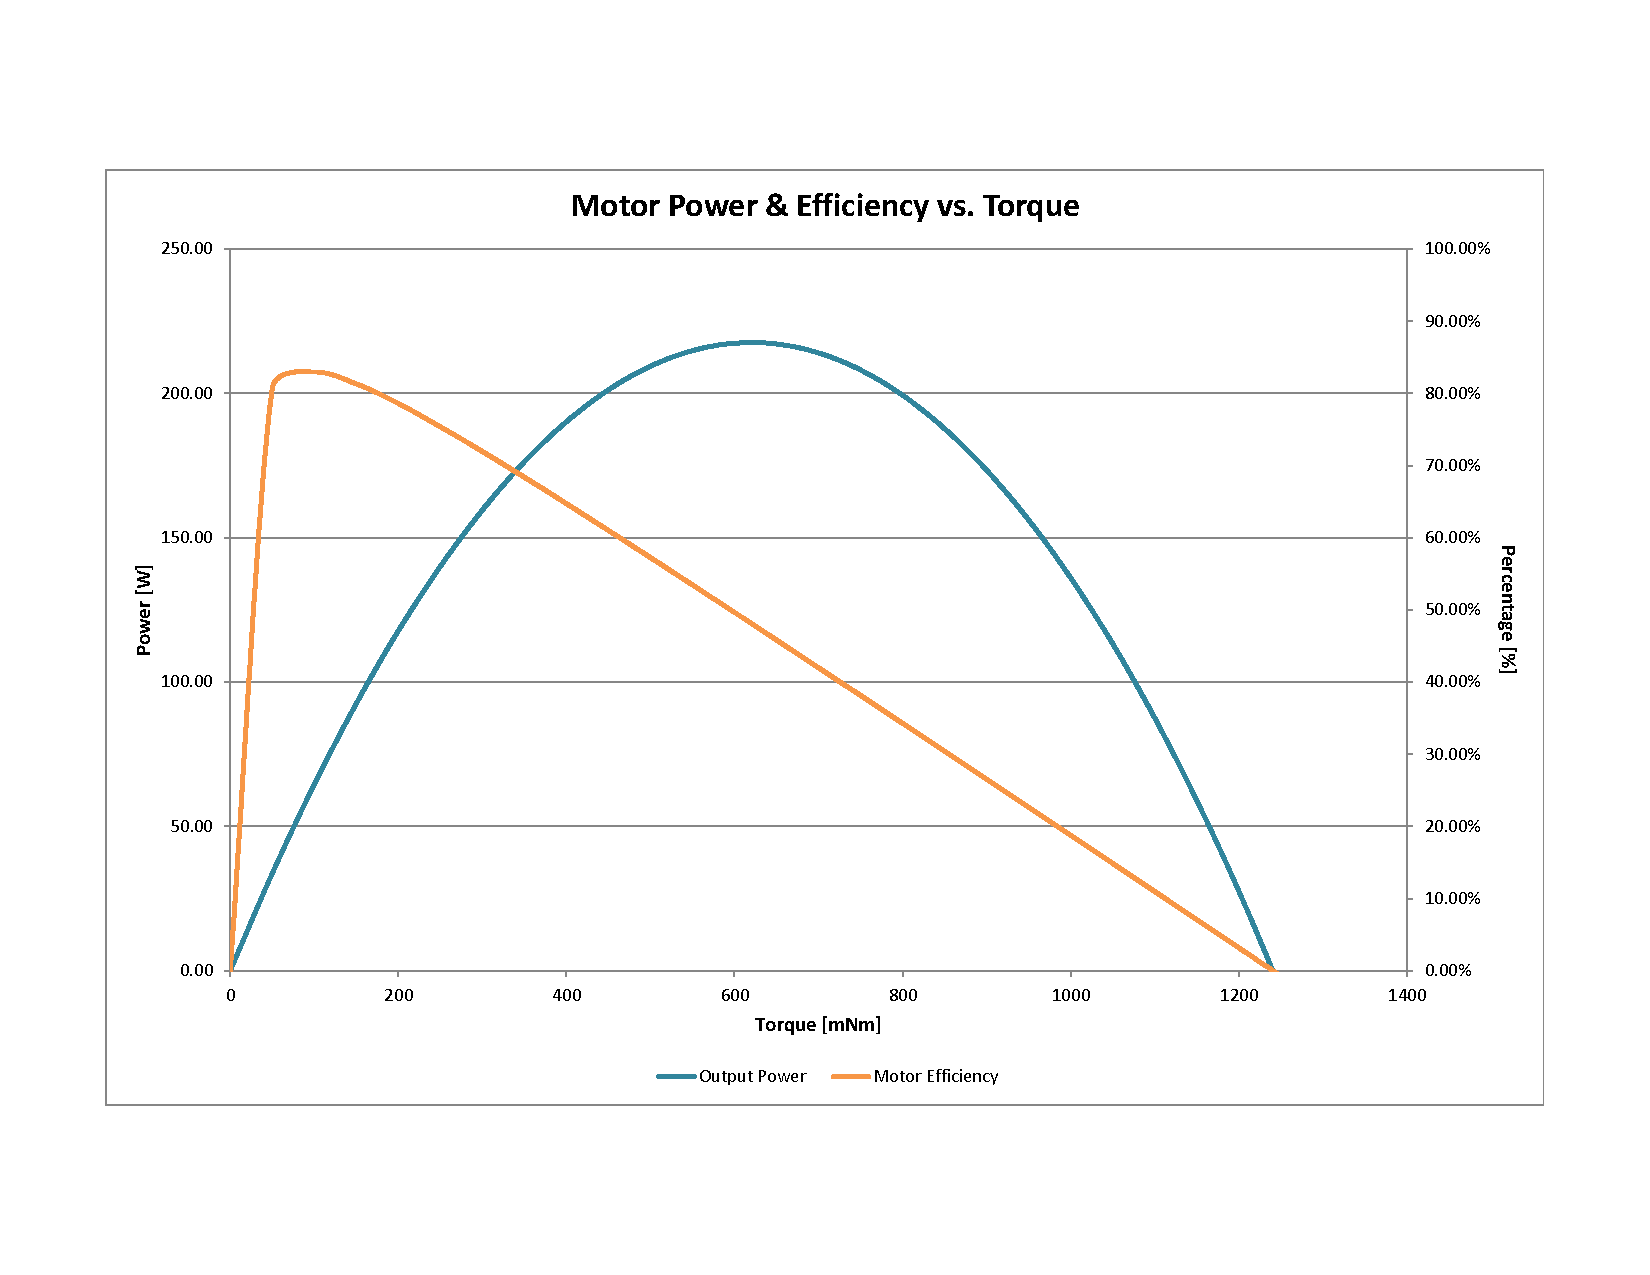
\includegraphics[scale=0.6]{fig/ch5/motor2.pdf}
	\end{center}
  \caption{Micromo 3257CR Coreless DC Motor: Power and Efficiency vs Torque}
\end{figure}

% subsection power_and_efficiency_analysis (end)

\subsection{Thermal Analysis} % (fold)
\label{sub:thermal_analysis}
As mentioned previously, out of the initial design specifications the motor selection process is based on the continuous or average torque loading on the joints. However, during each gait cycle the torque peaks as soon as impulsive forces are experienced from the environment (i.e. heel-strike). While these peaks may be outside of the motors continuous operating range for a very short period of time, the heat generated inside the motor core can build up and cause significant damage. Another consideration is the effect of thermal build up of the motor under continuous use at the specification of 14Nm. Therefore it is necessary to generate thermal plots alongside the torque-speed analysis to verify that the selected motors can withstand the temperature rise due to its operation. Given an assumed value for the ambient temperature, the total temperature of the motor can be calculated as: 

\begin{equation}
	T_{total} = T_{ambient} + T_{inc}
\end{equation}

Where the temperature increase inside the motor core is provided by the following relationship: 

\begin{equation}
	T_{inc} = I^{2}R \times (R_{th1} + R_{th2})
\end{equation}

Note that $I$ and $R$ is the current through and the resistance of the motor windings, respectively. Constants $R_{th1}$ and $R_{th2}$ are specified by the motor manufacturer. 


\begin{figure}[!ht]
	\begin{center}
    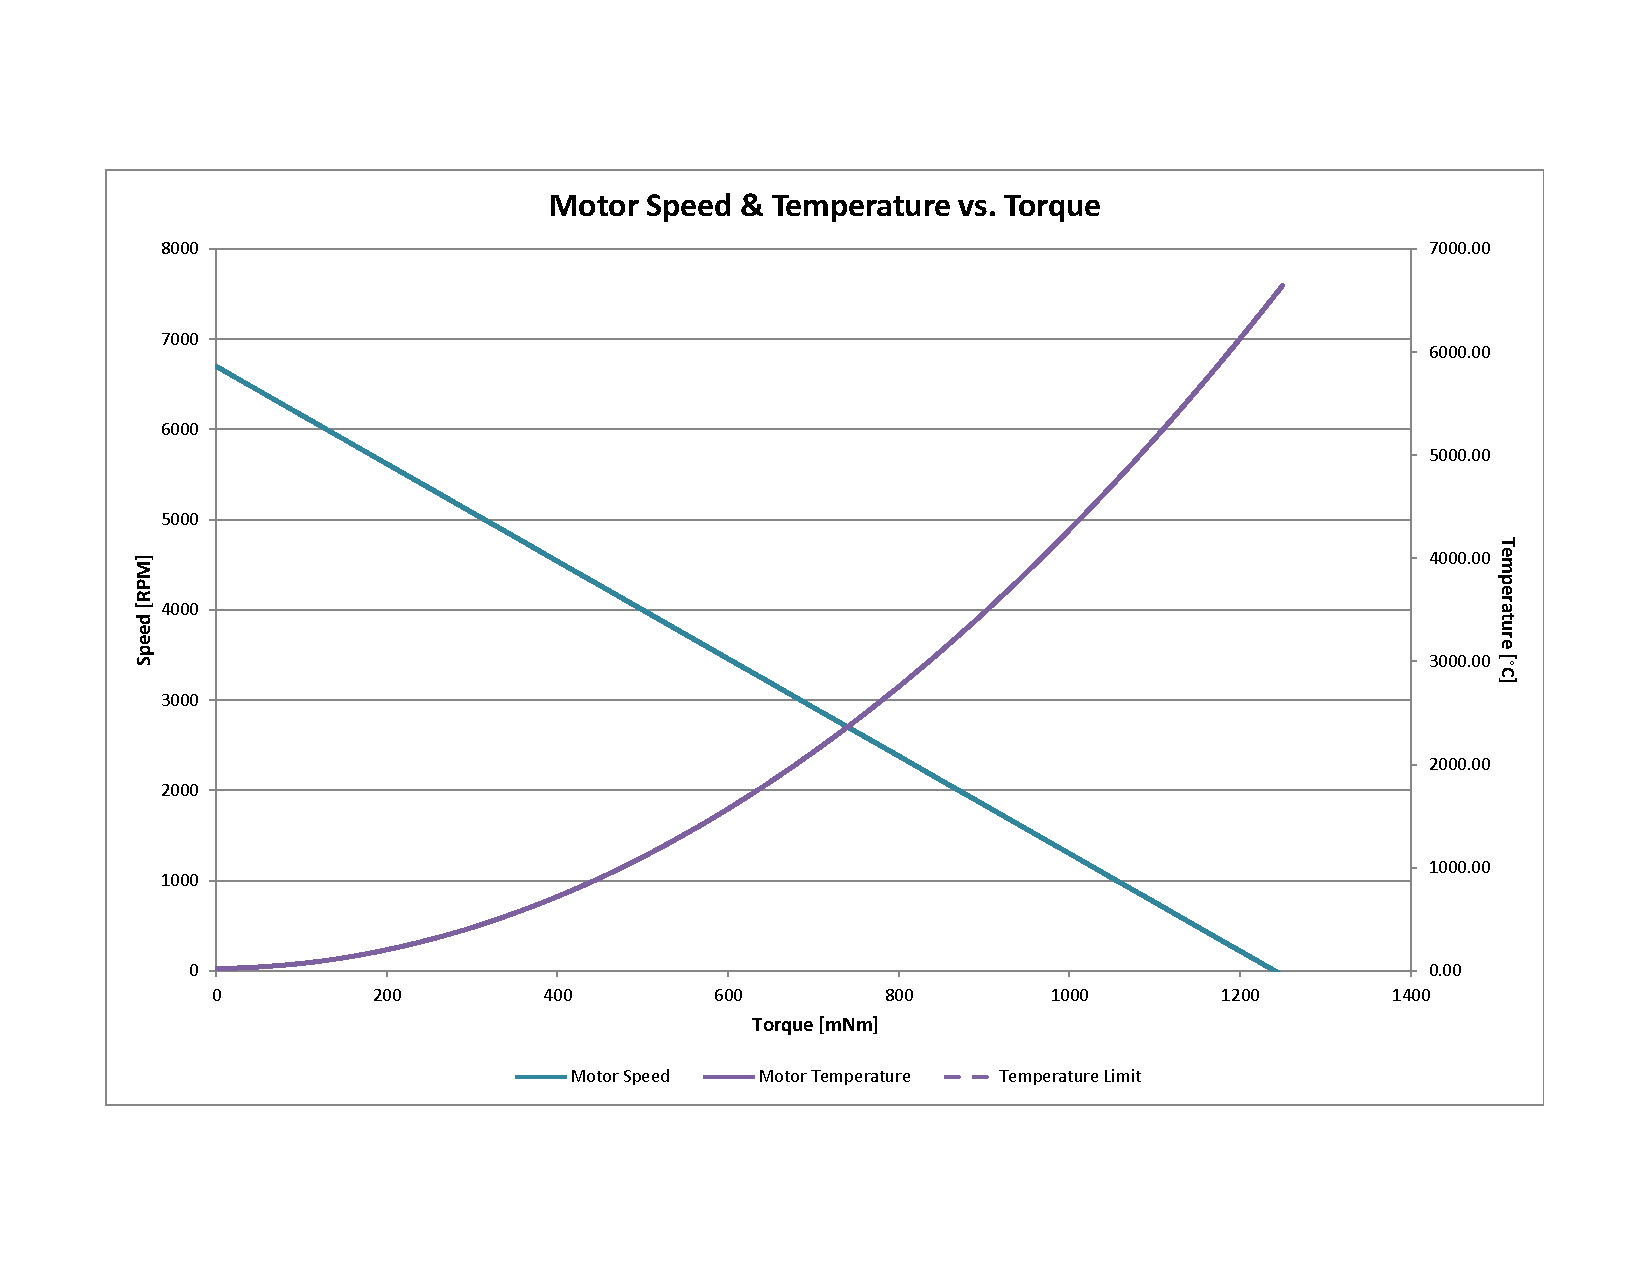
\includegraphics[scale=0.6]{fig/ch5/motor3.pdf}
	\end{center}
  \caption{Micromo 3257CR Coreless DC Motor: Speed and Temperature vs Torque}
\end{figure}
% subsection thermal_analysis (end)

\subsection{Design Considerations} % (fold)
\label{sub:design_considerations}
Aside from the torque-speed, power, efficiency and thermal analysis, there are several other factors which come into the design procedure for selecting the drivetrain components. These considerations pertain to the secondary objective to minimize the overall weight of the drivetrain components while having as much mass as possible shifted upwards in the structure. Out of the two components used for the drivetrain, the majority of the weight comes from the actual coreless DC motor so it is desirable to select smaller motors and meet the specified torque requirements by means of increasing the reduction ratio on the matching gearhead. Another consideration is the physical size of the motor itself, as the diameter and length of each motor vary significantly between different offerings. Since gearheads are coupled directly onto the motor shaft, the complete drivetrain assembly is usually quite long. While these factors are not critical design considerations, there were used as a means for comparison if two drivetrain selections were comparable in terms the primary considerations.% subsection design_considerations (end)


\subsection{Final Configurations} % (fold)
\label{sub:final_configurations}

Given the considerations and the points of analysis stated in the previous sections, a coreless DC motor from the Micromo Solutions catalog was selected. This motor achieved all of the primary design considerations in terms of meeting the average torque requirements and maintaining operation within a stable thermal region. The following charts illustrate the characteristics at the output of the motor shaft. 

Coupled with the motor is a matching precision gearhead which provides the torques mentioned in the specifications with some added buffer. The reduction ratio of the gearheads was selected such that larger reduction ratios within the same model could be selected if it was determined that the revised design had an increase in torque loading at the joints which the initial selection was unable to meet. The charts shown above illustrate the characteristics at the output of the gearhead shaft.

\begin{figure}[!ht]
	\begin{center}
    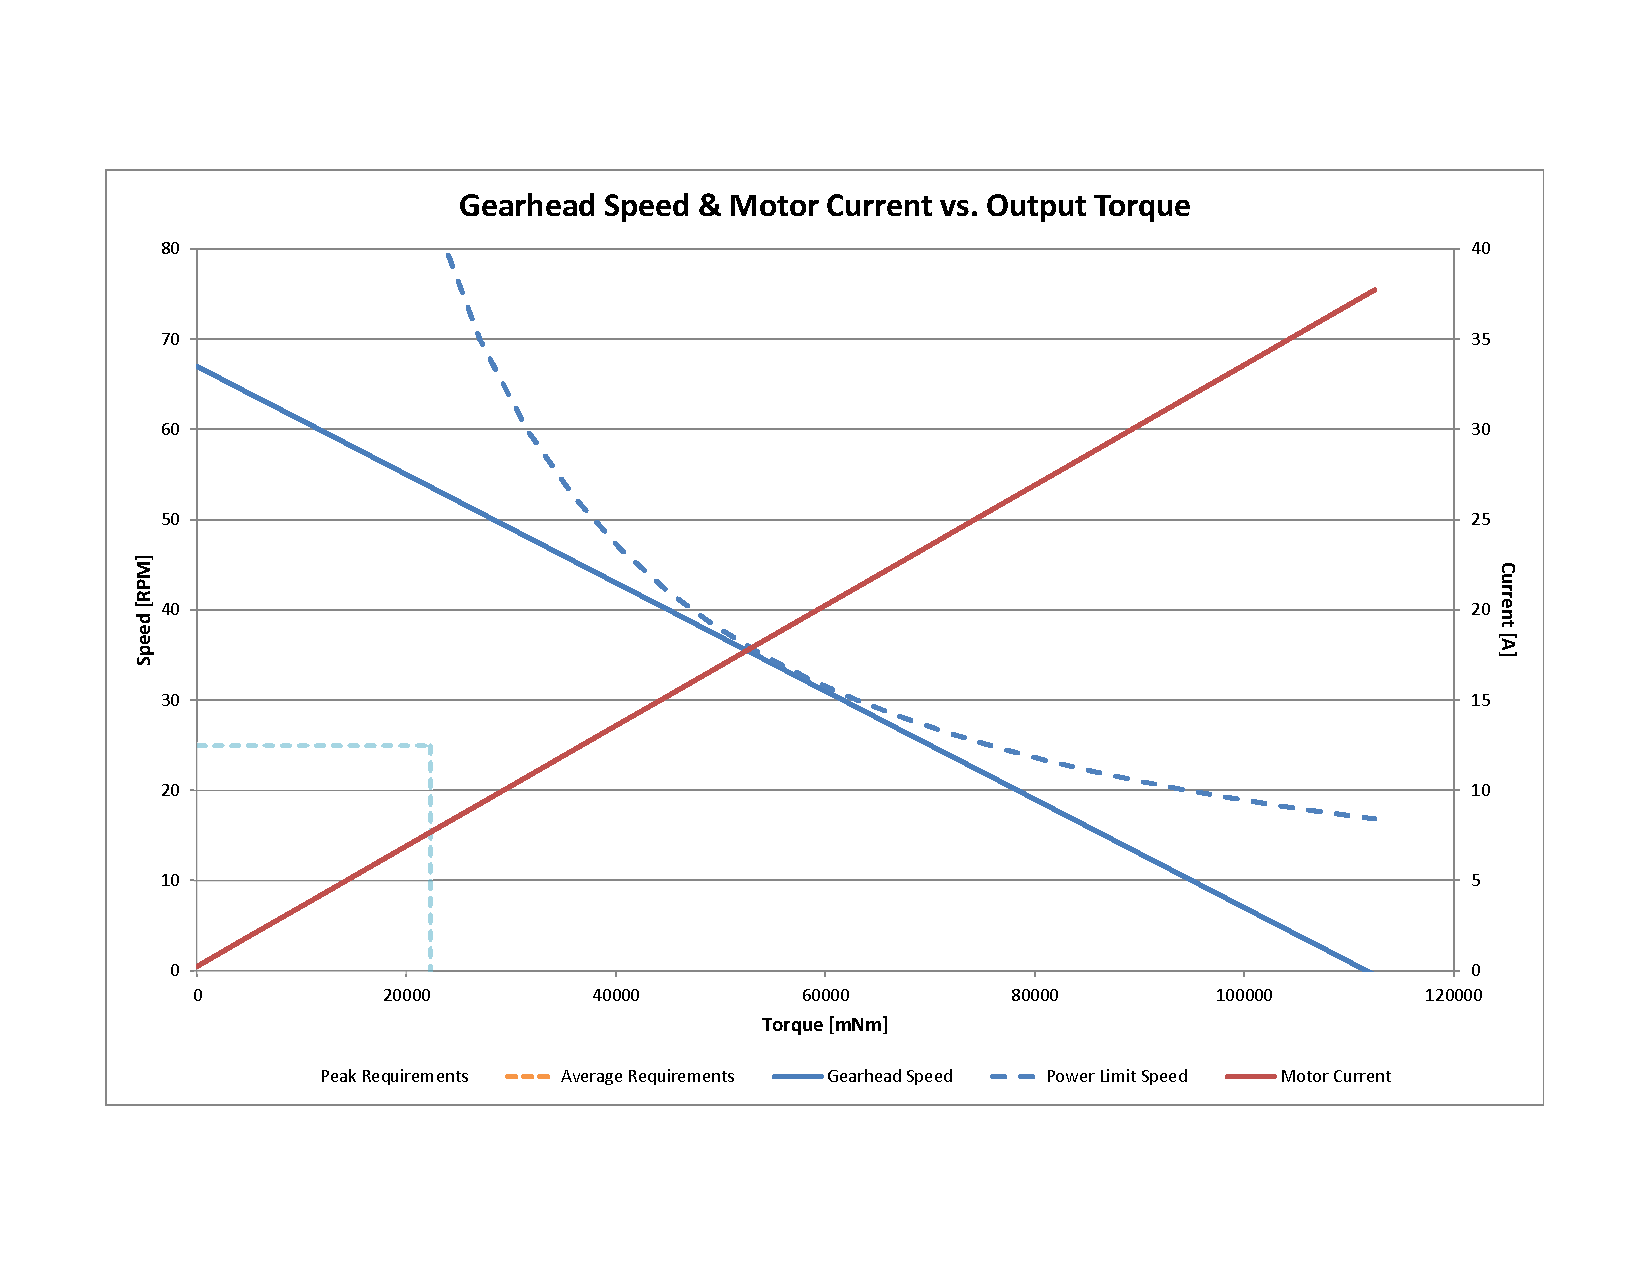
\includegraphics[scale=0.6]{fig/ch5/gearhead1.pdf}
	\end{center}
  \caption{Micromo 38A Precision Gearhead: Speed and Current vs Torque}
\end{figure}

It was mentioned previously that the torque demands vary from joint to joint. However, to limit the number of motor selections and to simplify the overall mechanical design the number of motors used throughout the complete biped is limited to two configurations. The larger configuration is to be used at joints which require higher joint torques and/or velocities, whereas the lower configuration is used in joints with lower demands. Ultimately, the following two configurations are selected on the basis of meeting torque and velocity requirements. 


\begin{table}[!h]
  \centering
  \caption{Higher configuration of motor and gearhead combination from Micromo.}
    \begin{tabular}{lcccc}
    \addlinespace
    \toprule
    \textbf{Model} & \textbf{Mass} & \textbf{Length} & \textbf{Stall Torque} & \textbf{Max Power}\\
    \midrule
    3257CR 12V Motor	&	242g	&	57mm	&	0.547Nm		&	84.50W	\\
    38A 240:1 Gearhead	&	410g	&	80mm	&	20.0Nm		&	-	\\
    \bottomrule
    \end{tabular}%
  \label{tab:higherconfig}%
\end{table}%



\begin{table}[!h]
  \centering
  \caption{Lower configuration of motor and gearhead combination from Micromo.}
    \begin{tabular}{lcccc}
    \addlinespace
    \toprule
    \textbf{Model} & \textbf{Mass} & \textbf{Length} & \textbf{Stall Torque} & \textbf{Max Power}\\
    \midrule
    3242CR 12V Motor	&	172g	&	42mm	&	0.193Nm		&	27.30W	\\
    32A 68:1 Gearhead	&	240g	&	57mm	&	6.0Nm		&	-	\\
    \bottomrule
    \end{tabular}%
  \label{tab:lowerconfig}%
\end{table}%


From the human gait analysis section, it was determined that the only joint which uses the lower configuration (Table \ref{tab:lowerconfig}) is the ankle roll DOF. The remaining 6 DOF in each leg use the higher configuration (Table \ref{tab:higherconfig}) due to torque and/or velocity demands.
% subsection final_configurations (end)


% section drivetrain (end)

% chapter design (end)